\documentclass[12pt,a4paper,final]{report}
\usepackage[utf8]{inputenc}
\usepackage[spanish]{babel}
\usepackage{amsmath}
\usepackage{amsfonts}
\usepackage{amssymb}
\usepackage{graphicx}
\usepackage{subcaption}
\usepackage{tocloft}
\usepackage{listings}
\usepackage[sort&compress,square,comma,authoryear]{natbib}
\bibliographystyle{unsrtnat}

\renewcommand\cftchapdotsep{\cftdotsep}

\author{Mingari L.}
\title{Productos de datos Lidar para dispersión elástica}
\begin{document}

\begin{titlepage}
	\centering
	\includegraphics[width=0.4\textwidth]{figures/savernet} \hfill
    \includegraphics[width=0.5\textwidth]{figures/smn}\par \vspace{1cm}
	{\scshape\LARGE Proyecto SAVERNet \par}
	\vspace{1cm}
	{\scshape\Large Informe técnico\par}
	\vspace{1.5cm}
	{\huge\bfseries Productos de datos Lidar para dispersión elástica\par}
	\vspace{2cm}
	{\Large\itshape Leonardo A. Mingari\par}
	{E-mail: lmingari@gmail.com\par}
	\vfill
	\textsc{CONICET}\par
	\textsc{Servicio Meteorológico Nacional}\par
	\textsc{Instituto de Física de Buenos Aires}\par
	\vfill
	% Bottom of the page
	{\large \today\par}
\end{titlepage}

	\tableofcontents
	\chapter{Introducción}
	En este informe se describen los producto obtenidos a partir de los datos Lidar para los canales elásticos $1064 \, nm$ y $532 \, nm$ en sus dos componentes perpendiculares. Uno de los objetivos más importante de estos productos es caracterizar la presencia de aerosoles en la atmósfera, típicamente por medio del coeficiente de extinción o atenuación de aerosoles. No obstante, la atenuación debido a aerosoles no puede ser derivada directamente a partir de la señal lidar de retrodispersión elástica, ya que es necesario asumir un valor de la razón lidar, i.e., la relación entre los coeficientes de extinción y retrodispersión de aerosoles, en los algoritmos de inversión. En consecuencia, el método utilizado aquí conduce a una importante incerteza en los productos finales. Por otro lado, la sencillez del método empleado lo hace apropiado para emplearse en una implementación operacional, tal como es nuestro propósito final, mientras que los resultados obtenidos pueden aún proveer información valiosa.
	
	El métodos empleado está basado en los mismos principios empleados para obtener los productos operativos del National Institute for Environmental Studies, Japón. Una descripción de este método puede encontrarse en \citet{shimizu2017}. Estos algoritmos han sido desarrollados para ser aplicados en la red de instrumentos lidares de AD-Net (Asian dust and aerosol lidar observation network) y han sido probados y validados principalmente para al caso  de polvo mineral asiático. Nosotros hemos implementado estos productos con el fin de aplicarlos a la red de lidares ubicados en Argentina y Chile en el marco del proyecto SAVERNet (Sistema de Gestión de Riesgos Medioambientales Atmosféricos en Sudamérica). Si bien estos productos brindan información valiosa actualmente, aún se encuentran en fase experimental y se requiere al menos un año de pruebas y validaciones con datos externos independientes para adaptarlo a las condiciones de nuestra región.
	
	El desarrollo fue realizado utilizando el lenguaje de programación interpretado Python. Los productos de datos Lidar están disponibles en nivel 1 y 2 en forma operativa. Los datos de nivel 1 se obtienen hasta una altura de $18 \, km$ y los datos de nivel 2 hasta $9 \, km$ con una resolución vertical de $30 \, m$ en ambos casos. Para esto, los datos crudos a $7.5 \, m$ fueron resampleados previamente. A continuación se muestra la lista de productos disponibles:
	\begin{description}
		\item[Nivel 1:] Altura máxima $18 \, km$		
	\begin{itemize}
		\item Perfil de retrodispersión total atenuado a $532 \, nm$
		\begin{equation*}
		\beta'_{532}(z)
		\end{equation*}
		\item Perfil de retrodispersión total atenuado a $1064 \, nm$
		\begin{equation*}
		\beta'_{1064}(z)
		\end{equation*}
		
		Aquí se tiene en cuenta la contribución de aerosoles y moléculas y la transmisividad atmosférica
		\begin{equation*}
		\beta'(z)=(\beta_a(z) + \beta_m(z)) T_{\lambda}^2(z)
		\end{equation*}
		\item Perfil de retrodispersión total atenuado a $532 \, nm$ por componentes
		\begin{equation*}
		\beta'=\beta'_{\perp}+\beta'_{\parallel}
		\end{equation*}
		\item Razón de depolarización volumétrica a $532 \, nm$
		\begin{equation*}
		\delta_v = \dfrac{\beta_{\perp}}{\beta_{\parallel}}
		\end{equation*}
	\end{itemize}
	\item[Nivel 2:] Altura máxima $9 \, km$	
	
	\begin{itemize}
		\item Perfil del coeficiente de retrodispersión de aerosoles a $532 \, nm$ por el método de Fernald
		\begin{equation*}
		\beta_a(z)
		\end{equation*}
		\item Razón de depolarización de aerosoles a $532 \, nm$
		\begin{equation*}
		\delta_a
		\end{equation*}
		\item Coeficiente de extinción o atenuación de aerosoles total y de partículas no esféricas a $532 \, nm$ 
		\begin{equation*}
		\alpha_a = \alpha_s + \alpha_d
		\end{equation*}
	\end{itemize}
	\end{description}
	
	En la Fig.~\ref{fig:products} se muestra un ejemplo de algunos de los productos obtenidos para la estación Comodoro Rivadavia en junio de 2017.
	
	\begin{figure}
		\begin{subfigure}{\textwidth}
		  \centering
		  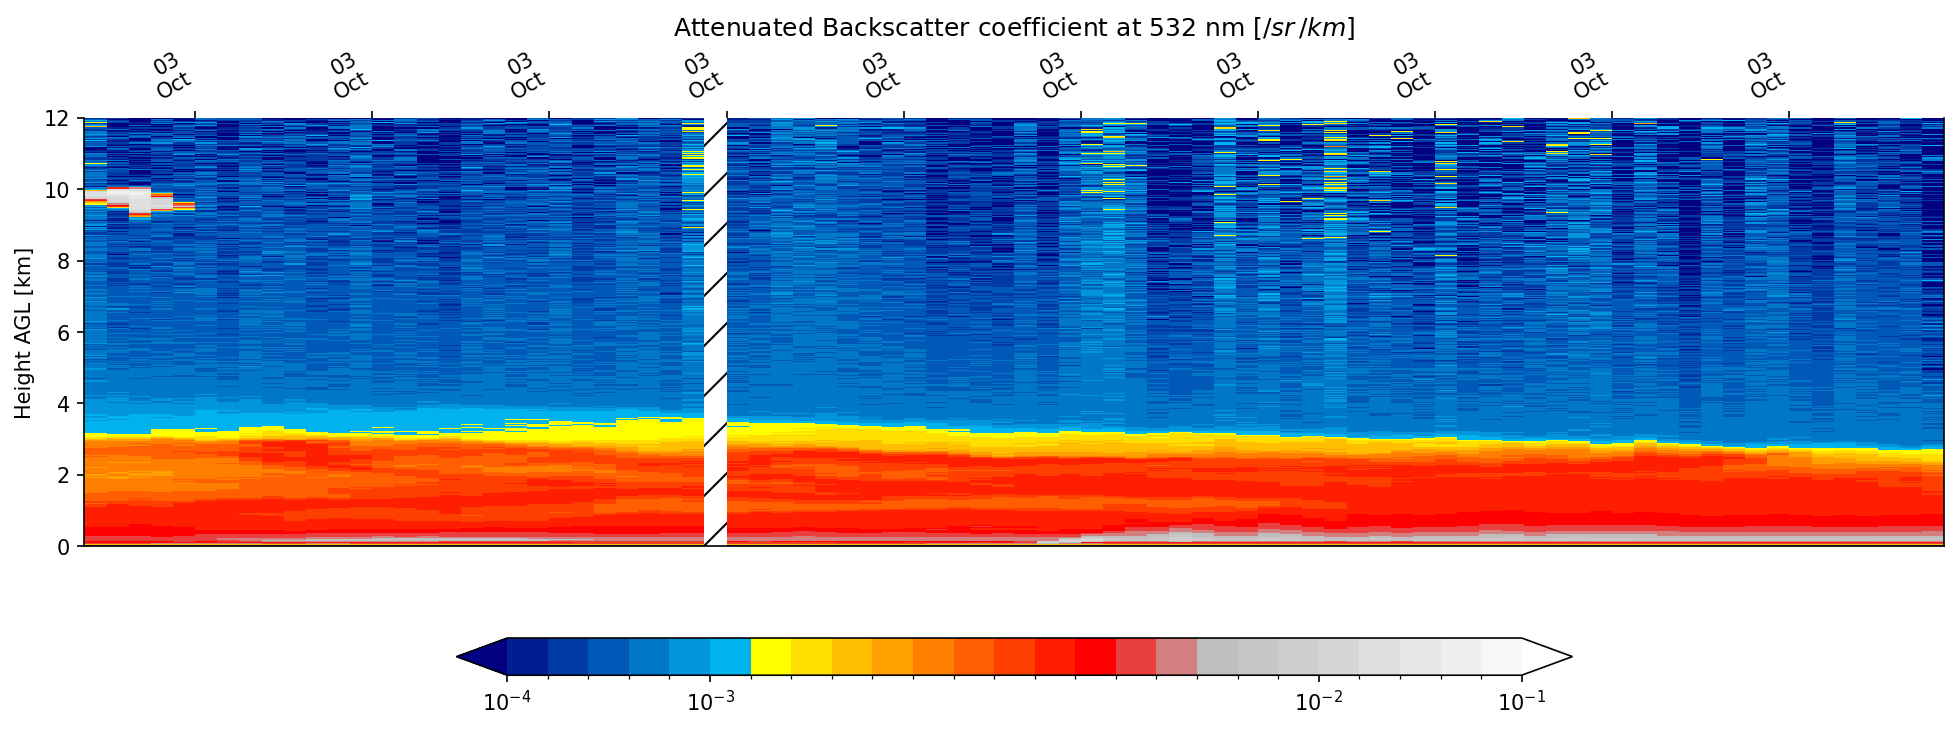
\includegraphics[width=0.6\textwidth]{figures/absc_vis}
		\end{subfigure}

		\begin{subfigure}{\textwidth}
			\centering
			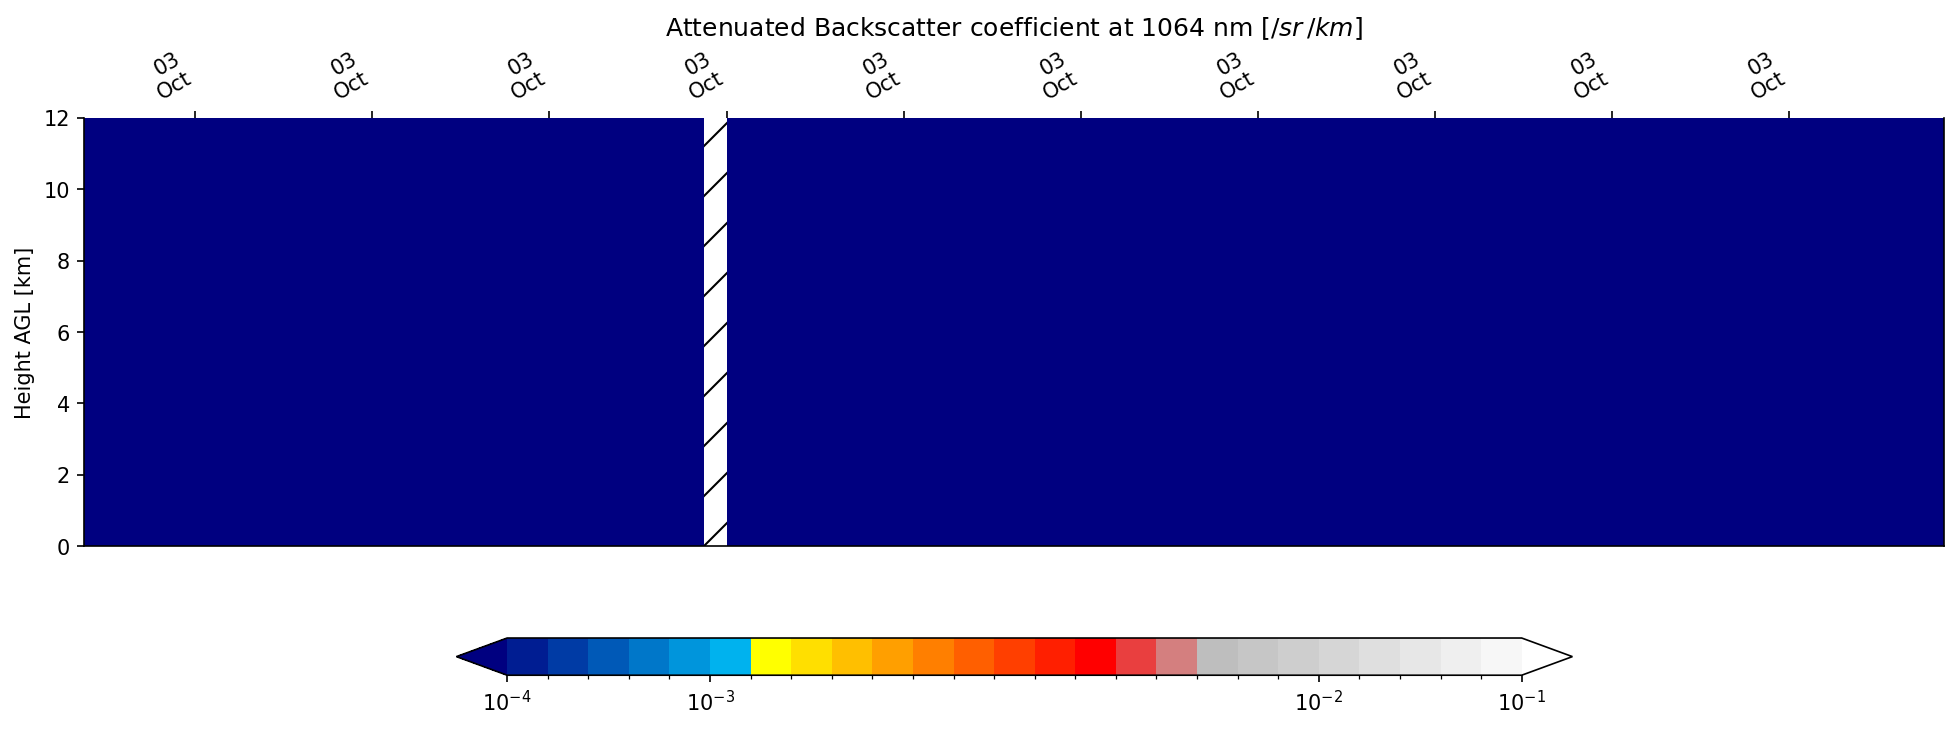
\includegraphics[width=0.6\textwidth]{figures/absc_ir}
		\end{subfigure}
		
		\begin{subfigure}{\textwidth}
			\centering
			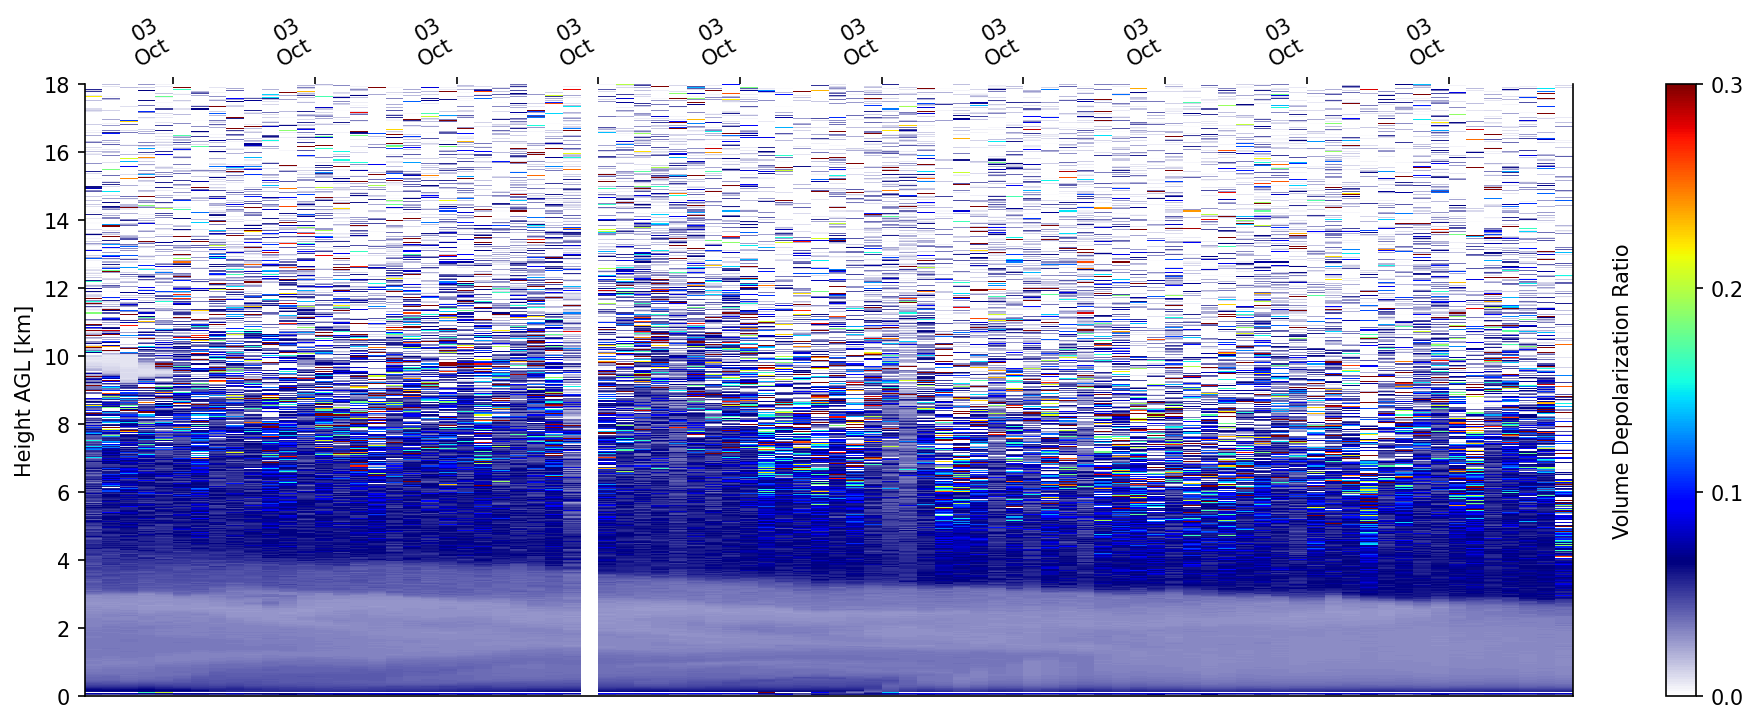
\includegraphics[width=0.6\textwidth]{figures/dep}
		\end{subfigure}

		\begin{subfigure}{\textwidth}
			\centering
			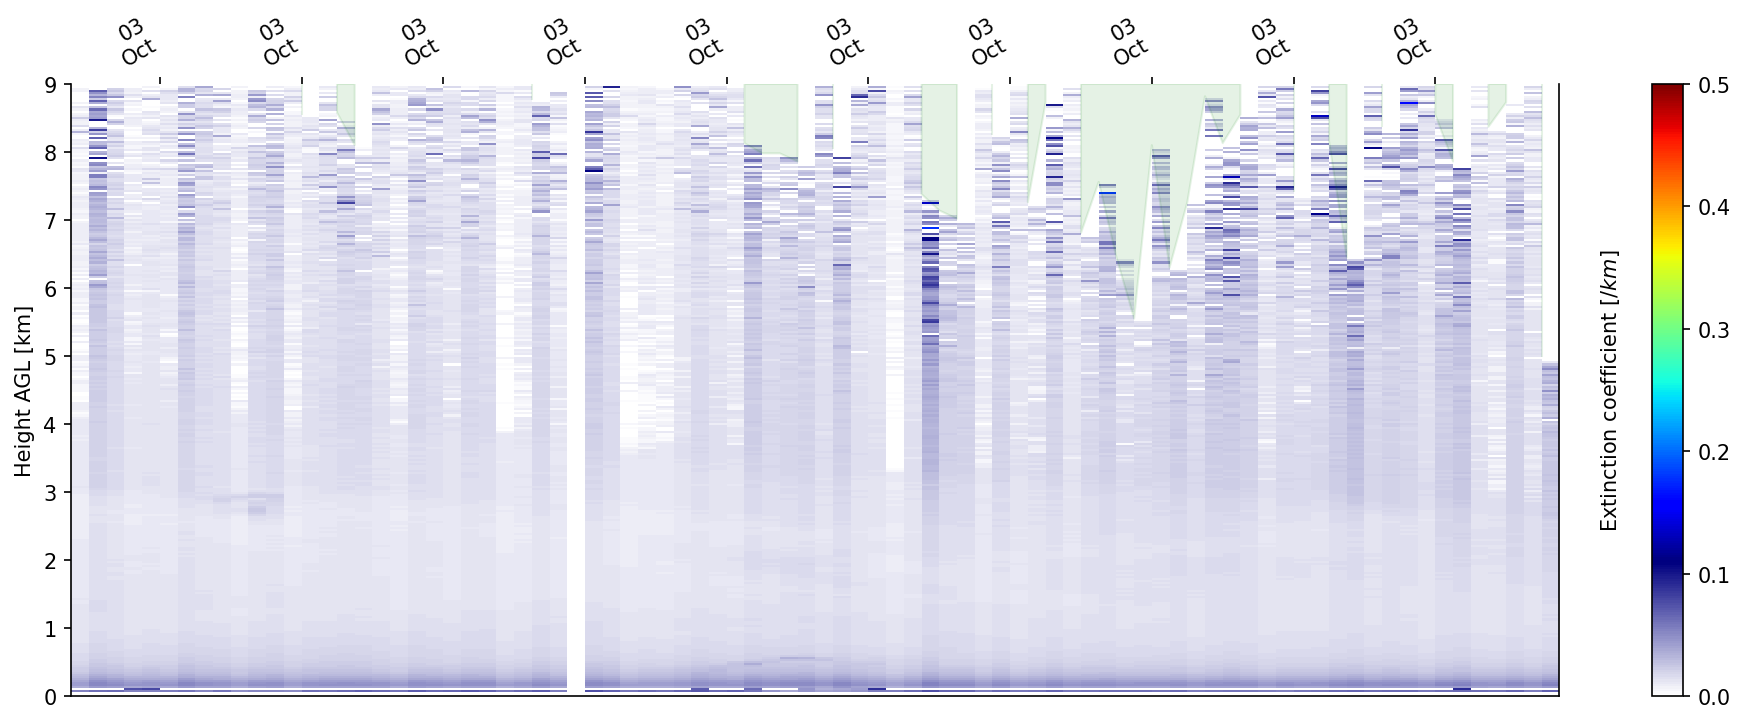
\includegraphics[width=0.6\textwidth]{figures/dust}
		\end{subfigure}
		
		\begin{subfigure}{\textwidth}
			\centering
			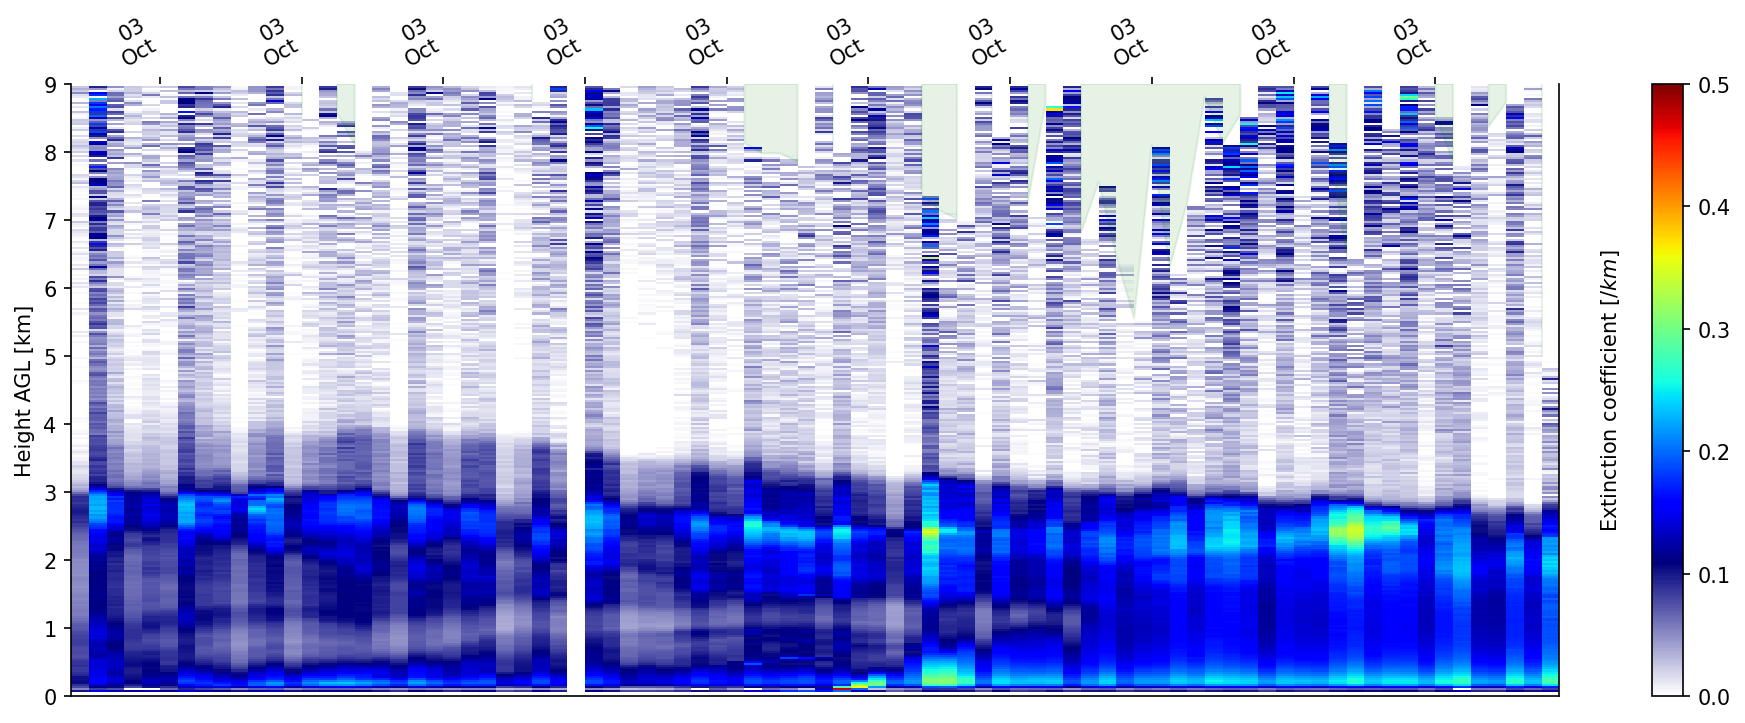
\includegraphics[width=0.6\textwidth]{figures/sphere}
		\end{subfigure}
		\caption{Ejemplos de productos de datos Lidar para la estación Comodoro Rivadavia en junio de 2017.}
		\label{fig:products}
	\end{figure}
	
	\chapter{Código Python}
	La estructura del código Python se muestra en la Fig.~\ref{fig:program}. El programa fue probado para la versión \emph{Python 2.7.12} en linux. El programa principal \emph{main.py} utiliza los módulos de los paquetes \emph{Reading} e \emph{Inversion}. Para su ejecución, en primer lugar se deben dar permisos de ejecución
	\begin{lstlisting}[language=bash]
	$ chmod +x main.py
	\end{lstlisting}	
	y luego ejecutar el código con la siguiente línea
	\begin{lstlisting}[language=bash]
	$ ./main.py Station
	\end{lstlisting}
	donde los posibles valores de \emph{Station} son:
	\begin{itemize}
		\item Aeroparque
		\item Bariloche
		\item Cordoba
		\item Gallegos
		\item Neuquen
		\item Punta
		\item Tucuman
	\end{itemize}
	
	El programa busca en su directorio un fichero de configuración \emph{parameters.cfg} en donde se definen todos los parámetros de la corrida. Cada parámetro tiene un valor por defecto definido en el bloque \emph{Default}. Estos valores pueden ser modificados dentro del bloque \emph{Station} específico para cada estación (ver Sec.~\ref{ch:appendix} para más información sobre el formato de este fichero). Asimismo, durante la ejecución del programa se leen ficheros con las correcciones de solapamiento y potencia, cuyos nombres se definen en el bloque \emph{Paths} del fichero de configuración.
	
	\begin{figure}
		\begin{center}
			\includegraphics[width=0.7\textwidth]{figures/program}
		\end{center}
		\caption{
			Estructura del código Python.
		}
		\label{fig:program}
	\end{figure}
	
	En primer lugar se leen los datos binarios y se convierten a formato NetCDF mediante el módulo \emph{ReadRaw}. Para esto, los datos crudos son promediados temporalmente sobre un periodo de tiempo definido por el parámetro \emph{sampling} en el fichero de configuración. Se recomienda el valor \emph{sampling=15} dado que la mayoría de las estaciones reinician las mediciones cada 15 minutos, excepto Córdoba, donde se realizan mediciones continuas y es posible definir un menor sampling hasta un minuto ($sampling \ge 1$).
	
	Posteriormente, se llama al módulo \emph{Invert532}, el cual se encarga de realizar las calibraciones, la detección de nubes y la determinación de la altura de inversión. Finalmente, se cargan los perfiles moleculares y se lleva a cabo la inversión de la señal. Los resultados se grafican y se guardan en un fichero de salida en formato NetCDF. Una información detallada de las variables que se guardan en este fichero pueden obtenerse con el comando \emph{ncdump}. Por ejemplo:
	\begin{lstlisting}[basicstyle=\footnotesize, language=bash]
	$ ncdump -h cfeb2017.nc 
	netcdf cfeb2017 {
	dimensions:
	time = UNLIMITED ; // (1824 currently)
	alt1 = 600 ;
	alt2 = 300 ;
	variables:
	float time(time) ;
	time:units = "minutes since 2017-02-01 00:00:00" ;
	time:description = "time after 0000UTC" ;
	float alt1(alt1) ;
	alt1:units = "km" ;
	alt1:description = "altitude" ;
	float alt2(alt2) ;
	alt2:units = "km" ;
	alt2:description = "altitude" ;
	float bsc532(time, alt1) ;
	bsc532:units = "/sr /km" ;
	bsc532:description = "Attenuated Backscatter coefficient (532 nm)" ;
	float bsc1064(time, alt1) ;
	bsc1064:units = "/sr /km" ;
	bsc1064:description = "Attenuated Backscatter coefficient (1064 nm)" ;
	float dep(time, alt1) ;
	dep:units = "" ;
	dep:description = "Volume Depolarization ratio" ;
	float ext_d(time, alt2) ;
	ext_d:units = "/km" ;
	ext_d:description = "Extinction coefficient - Non spherical particles" ;
	float ext_s(time, alt2) ;
	ext_s:units = "/km" ;
	ext_s:description = "Extinction coefficient - Spherical particles" ;
	float zb(time) ;
	zb:units = "km" ;
	zb:description = "Cloud Bottom" ;
	float zt(time) ;
	zt:units = "km" ;
	zt:description = "Cloud Top" ;
	float zinv(time) ;
	zinv:units = "km" ;
	zinv:description = "Inversion height" ;
	
	// global attributes:
	:TITLE = "LIDAR products" ;
	:YEAR = 2017 ;
	:MONTH = 2 ;
	:DAY = 1 ;
	:STATION = "c" ;
	}
	\end{lstlisting}
	
	\chapter{Descripción de los algoritmos}
	El algoritmo empleado sigue la estructura descripta por \citet{shimizu2017}. En las figuras~\ref{fig:scheme1}-\ref{fig:scheme3} se muestra un esquema simplificado del mismo.
	
	En primer lugar, se extrae el background de la señal y se corrige en rango. Posteriormente, se realiza la corrección con el factor de solapamiento, el cual es determinado experimentalmente en condiciones atmosférica en que se encuentra una PBL bien desarrollada, debido a que en estas condiciones se espera una distribución homogénea de aerosoles en las capas bajas. Eventualmente, son necesarias también correcciones por discontinuidades en la potencia recibida. Para la calibración se requiere conocer la razón de sensibilidad entre los PMTs de los canales visibles dado que el canal perpendicular se suele configurar con una mayor sensibilidad  para compensar la señal más débil que recibe en general. 
	
	Para la calibración del canal visible se utiliza el método del histograma, ya que la retrodispersión molecular es dominante en este rango de alturas ($1200-6000 \, m$) y puede ser  estimada aproximamente. Para el canal infrarrojo, la calibración se realiza asumiento un color ratio igual a uno en nubes meteorológicas. En la Fig.~\ref{fig:scheme1} se observa un esquema del procedimiento empleado para la calibración.
	
	\begin{figure}[t]
		\begin{center}
			\includegraphics[width=0.65\textwidth]{figures/fig01}
		\end{center}
		\caption{
			Procedimiento empleado en el proceso de calibración.
		}
		\label{fig:scheme1}
	\end{figure}
	
	En la Fig.~\ref{fig:scheme2} se muestran los pasos previos a aplicar el algoritmo de inversión. En primer lugar, se descartan condiciones lluviosas, con niebla, nieve, etc. El algoritmo tampoco puede ser aplicado a capas con nubes, con lo cual es necesario aplicar un método de detección de nubes previamente basado en el gradiente de la señal. Entonces la altura de inversión se define debajo de las nubes, mientras que si no hay nubes es definido a una altura máxima de $9 \, km$. Sin embargo, esta altura puede ser menor dependiendo de la relación señal/ruido de la señal. Posteriormente, la señal es promediada verticalmente hasta una resolución vertical de $30\,m$ para aumentar la relación señal ruido.
	
	\begin{figure}[t]
		\begin{center}
			\includegraphics[width=0.8\textwidth]{figures/fig02}
		\end{center}
		\caption{
			Pasos previos a aplicar el algoritmo de inversión y determinación de la altura de inversión.
		}
		\label{fig:scheme2}
	\end{figure}
	
	Finalmente, la ecuación Lidar para dispersión elástica se resuelve para dos componentes, i.e., aerosoles y moléculas, por el método de Fernald (ver Sec.~\ref{ch:inversion}). Para esto, se calculan previamente los perfiles moleculares para una atmósfera estándar. Para realizar la inversión de la señal lidar, se asume que la contribución de aerosoles a la señal retrodispersada es mucho más pequeña que la contribución molecular en la altura de inversión y se itera hacia abajo usando la Eq.~\ref{eq:discret_beta}, descripta en la Sec.~\ref{ch:inversion}. A partir del método de Fernald se obtienen los perfiles de los coeficientes de extinción y retrodispersión de aerosoles.
	
	El valor inicial del coeficiente de extinción en la altura de inversión es desconocido y se asume muy pequeño. Debido a esta incerteza y a que la señal a esta altura puede ser muy ruidosa, el algoritmo de inversión puede dar lugar a resultados inconsistentes (en concreto, $\alpha_a<0$). En este caso, el algoritmo de inversión se aplica iterativamente con valores iniciales de $\alpha_a$ progresivamente más grandes hasta que la condición $\alpha_a(z)>0$ es satisfecha. Cabe aclarar que este estrategia no es rigurosa, y ésta es una de las fuentes de error más importantes del método.
	
	La razón de depolarización de aerosoles ($\delta_a$) es una magitud clave para ponderar la presencia de partículas no esféricas, e.g., polvo mineral o cenizas volcánicas. Por otra parte, la contribución de partículas esféricas se ha atribuido a la presencia de sulfato, nitrato y otras especies de origen antropogénico \citep{shimizu2017}. 
	
	La contribución de las partículas esféricas y no esféricas a los perfiles del coeficiente de extinción se calculan a partir de $\delta_a$. El coeficiente de extinción de partículas no esféricas es la magnitud más significativa para realizar comparaciones con las salidas de los modelos de dispersión de polvo mineral o cenizas volcánicas. A menudo se asume que existe una relación lineal entre estas variables.
	
	Por último, las constantes de calibración son re-calculadas  para obtener una mejor estimación de los coeficientes de retrodispersión atenuados. Los datos son graficados y guardados en los ficheros de salida.
	
	Todo el procedimiento es repetido operativamente cada una hora para todas las estaciones si nuevos datos son recibidos.
	
	\begin{figure}[t!]
	\centering
	\includegraphics[width=0.6\textwidth]{figures/fig03}
	\caption{
	Aplicación del algoritmo de inversión y cálculo de la contribución de partículas no esféricas.
	}
	\label{fig:scheme3}
	\end{figure}
	
	\chapter{Algoritmo de inversión: Método de Fernald}
	\label{ch:inversion}
	El algoritmo que se describe a continuación permite obtener el coeficiente de retrodispersión para aerosoles utilizando una técnica muy sencilla a partir de la señal corregida en rango.
	
	La ecuación Lidar para dos clases de dispersores, i.e., aerosoles y moléculas, viene dada por:
	\begin{equation}
	P(Z) = EC Z^{-2} [\beta_1(Z) + \beta_2(Z)] T_1^2(Z) T_2^2(Z)
	\end{equation}
	donde $P(Z)$ es la señal recibida, $E$ es proporcional a la energía transmitida, $C$ es la constante de calibración, $\beta=\beta_1 + \beta_2$ es el coeficiente de retrodispersión total, $T_1$ y $T_2$ son las transmitancias de aerosoles y moléculas, respectivamente, dadas por:
	\begin{equation}
	T_i(Z) = \exp \left(-\int_0^z \alpha_i dz \right)
	\end{equation}
	siendo $\alpha_i(Z)$ el coeficiente de extinción de la clase $i$.
	
	La principal hipótesis de este algoritmo es que la razón Lidar para aerosoles
	\begin{equation}
	S_1=\dfrac{\alpha_1(Z)}{\beta_1(Z)}
	\end{equation}
	no depende de la altura. Esto es aproximadamente válido si la distribución de tamaños y la composición de los aerosoles no cambian con la altura, y la variaciones en la retrodispersión se deben únicamente a cambios en la densidad de aerosoles. Nosotros asumimos un valor $S_1=50  \, sr$. 
	
	La ecuación Lidar escrita en términos de la señal corregido en rango, $X(Z)=P(Z) Z^2$, da lugar a la ecuación integrodiferencial:
	\begin{equation}
	X(Z) = EC \beta(Z) \exp \left(  -2\int_0^Z S_1 \beta(Z') - (S_1 - S_2) \beta_2(Z') dZ' \right)
	\end{equation}
	Tomando el logaritmo y derivando obtenemos una ecuación diferencial de tipo Bernoulli
	\begin{equation}
	\frac{d}{dZ}\ln X(Z) =\dfrac{1}{\beta} \dfrac{d \beta}{dZ}-2(S_1 \beta - (S_1-S_2) \beta_2)
	\end{equation}
	que puede llevarse a una ecuación lineal haciendo el cambio de variables $ u=1/\beta $, 
	\begin{equation}
	\frac{du}{dZ}+uP(Z)=-Q(Z)
	\end{equation}
	con $P(Z)=\frac{d}{dZ}\ln X(Z)-2(S_1-S_2)\beta_2$ y $Q(Z)=2S_1$, cuya solución es
	\begin{equation}
	u(Z) \exp \left(\int_{Z_0}^{Z} P dZ'\right)-u(Z_0) = -\int_{Z_0}^{Z} Q \exp \left(\int_{Z_0}^{Z'} P dZ''\right) dZ'
	\end{equation}
	donde $Z_0$ es un rango de referencia.
	
	Entonces, la sección eficaz total de retrodispersión en $Z$ puede ser expresada como una función de las propiedades de dispersión en el rango de calibración ($Z_0$) y la capa entre $Z_0$ y $Z$:	
	\begin{equation}
	\beta(Z)=\frac{\displaystyle X(Z) \exp(-a(Z))}{\displaystyle \dfrac{X(Z_0)}{\beta(Z_0)}-2S_1 \int_{Z_0}^{Z} X(z)\exp(-a(z))dz}
	\label{eq:continuos_beta}
	\end{equation}
	con 
	\[ a(Z)=2(S_1-S_2)\int_{Z_0}^{Z} \beta_2 dz \]
	Esta ecuación, es formalmente igual a la empleada en de la red EARLINET \citep{bockmann2004}.
	
	En consecuencia, los perfiles de $\beta_1$ pueden obtenerse para todo $Z$ mediante un proceso iterativo  usando la Eq.~\ref{eq:continuos_beta} si es conocido $\beta_1$ en el rango de referencia $Z_0$. En la implementación numérica, esta ecuación se resuelve iterativamente en forma descendente a partir de una altura tope, que llamaremos altura de inversión. Para esto utilizaremos la versión discretizada de \citet{fernald1984}:
	
	\begin{equation}
	\beta_1(Z_{i-1}) = \dfrac
	{X(Z_{i-1}) \exp(a_{i-1,i})}
	{\dfrac{X(Z_{i})}{\beta_1(Z_{i})+\beta_2(Z_{i})}
		+S_1[X(Z_{i})+X(Z_{i-1}) \exp(a_{i-1,i})]\Delta Z}
	-\beta_2(Z_{i-1})
	\label{eq:discret_beta}
	\end{equation}
	con $a_{i,i+1}=(S_1-S_2)[\beta_2(Z_i)+\beta_2(Z_{i+1})]\Delta Z$
	
	\section{Perfiles moleculares}
	Para aplicar el método dado por la Eq.~\ref{eq:discret_beta} es necesario conocer la contribución molecular al coeficiente de retrodispersión o al coeficiente de extinción. Los parámetros que caracterizan la dispersión debido a moléculas pueden derivarse de la teoría de dispersión de Rayleigh. Según esta teoría la sección eficaz de dispersión total por molécula bajo condiciones estándares viene dada por \citep{bucholtz1995}
	\begin{equation}
	\sigma(\lambda) = 
	\dfrac{24 \pi^3}{\lambda^4 N_S^2} 
	\left( \dfrac{n_s^2-1}{n_s^2+2} \right)^2
	\dfrac{6+3 \rho_n}{6-7 \rho_n}
	\end{equation}
	siendo $\lambda$ la longitud de onda, $n_s$ el índice de refracción, $N_S$ la densidad numérica de moléculas para condiciones estándares y $\rho_n$ el factor de depolarización. Esta expresión muestra que existe una muy fuerte dependencia de la dispersión de Rayleigh con la longitud de onda. Por ejemplo, en la tabla~\ref{tab:rayleigh} se muestran algunos valores típicos para longitudes de ondas cercanas a las del lidar de dispersión elástica. Estos valores indican que el coeficiente de retrodispersión molecular para el canal infrarrojo es alredededor de dos órdenes de magnitudes más pequeño que para el ultravioleta.

    \begin{table}
    \centering
	\begin{tabular}{ c c c }
		\hline
		$\lambda$ & $\sigma$ & $\beta$ \\
		$(\mu m)$   & $(cm^2)$ & $(km^{-1})$ \\ \hline
		1000 & $4.010 \times 10^{-28}$ & $1.022 \times 10^{-3}$ \\
		550 & $4.509 \times 10^{-27}$ & $1.149 \times 10^{-2}$ \\
		320 & $4.279 \times 10^{-26}$ & $1.090 \times 10^{-1}$ \\ \hline
	\end{tabular}
   	\caption{Sección eficaz de dispersión total por molécula y coeficiente de dispersión  volumétrico total bajo condiciones estándares para dispersión de Rayleigh.}
   	\label{tab:rayleigh}
    \end{table}
	
    El coeficiente de dispersión  volumétrico total a una altitud $z$ puede estimarse usando la relación \citep{bucholtz1995}
	\begin{equation}
	\beta(z,\lambda) = N(z) \sigma (\lambda) = \dfrac{N_A P(z)}{R_a T(z)} \sigma (\lambda)
	\end{equation}	
	donde $N(z)$ es la densidad numérica de moléculas a la altitud $z$. Esta densidad se puede expresar en términos de la presión atmosférica, $P(z)$ (hPa), y la temperatura, $T(z)$ (K), usando la ecuación de los gases ideales, siendo $N_A = 6.02214 \times 10^{23} \, mol^{-1}$ el número de Avogadro y $R_a = 8.314472 ~ J K^{-1} mol^{-1}$ la constante de los gases. El espesor óptico de Rayleigh a la altitud $z_0$ puede calcularse por medio de la integral
	\begin{equation}
	\tau(z,\lambda)=\int_{z_0}^{\infty} \beta(z,\lambda) dz
	\end{equation}
	Nótese que $\beta$ tiene unidades de $m^{-1}$ y representa el coeficiente de extinción molecular según la teoría de Rayleigh.
	
	Nosotros usamos la expresión aproximada de $\sigma$ para una atmósfera estándar incluyendo la dependencia con la longitud de onda $\lambda$ ($nm$) dada por \citep{hostetler2006}
	\begin{equation}
	\sigma(\lambda) = 4.56 \times \left( \dfrac{550}{\lambda} \right)^4 \times 10^{-27} \, cm^2
	\end{equation}
	
	El coeficiente de retrodispersión puede obtenerse mediante la relación $\alpha_2 = S_2 \beta_2$. 	Según la teoría de dispersión de Rayleigh, el lidar ratio es aproximadamente
	 \begin{equation}
	 S_2 = 8 \pi /3 \, sr
	 \label{eq:s2}
	 \end{equation}
	
	\chapter{Discriminación de aerosoles no esféricos}
	A fin de discriminar entre aerosoles esféricos y no esféricos es útil emplear el concepto de razón de depolarización de aerosoles. Esta magnitud puede obtenerse a partir de la razón de depolarización volumétrica
	\begin{equation}
	\delta_v = \dfrac{\beta_{\perp}}{\beta_{\parallel}}
	\end{equation}	
	que depende de la densidad de aerosoles. La razón de depolarización de aerosoles se puede estimar a partir del coeficiente de retrodispersión de aerosoles usando la expresión
	\begin{equation}
	\delta_a = \dfrac{\delta_v (BR + BR \times \delta_m - \delta_m) - \delta_m}{BR - 1 + BR \times \delta_m - \delta_v}
	\end{equation}
	siendo $\delta_m=0.0044$ la razón de depolarización de moléculas, independiente de la altura, y $BR$ es la razón de dispersión:
	\[ BR=\dfrac{\beta_a + \beta_m}{\beta_m} \]
	
	La razón de depolarización de aerosoles permite  caracterizar la contribución de partículas no esféricas al coeficiente de extinción total. Para esto es necesario calcular la razón de mezcla (óptica) de  partículas no esféricas
	\begin{equation}
	R = \dfrac{(\delta_a - \delta_2)(\delta_1+1)}{(\delta_a+1)(\delta_1 - \delta_2)}
	\end{equation}
	siendo $\delta_1$ y $\delta_2$ la razón de depolarización de partículas no esféricas y esféricas, respectivamente. Los valores $\delta_1=0.35$ y $\delta_2=0.02$ fueron determinados empíricamente para polvo mineral asiático \citep{shimizu2004}.
	
	Entonces, es posible separar el coeficiente de extinción total a $532 \, nm$ en las componentes
	\begin{align}
	\alpha_d &= \alpha \times R \\
	\alpha_s &= \alpha \times (1-R)	
	\end{align}
	para partículas no esféricas y esféricas, respectivamente.
    
    \appendix
    \chapter{Formato del fichero de configuración}
    \label{ch:appendix}
    El fichero de configuración \emph{parameters.cfg} guarda todos los datos requeridos para la corrida: constantes físicas, parámetros experimentales, nombres de ficheros y directorios. Cada parámetro tiene un valor por default, que será usado por todas las estaciones, definido en el bloque \emph{Default}, salvo que sea explícitamente definido en un bloque de estación particular. Es este caso el bloque \emph{Station} tendrá prevalencia sobre el bloque \emph{Default}. El formato de este fichero puede verse en el siguiente ejemplo:
   
    \begin{verbatim}
    [DEFAULT]
    s1         = 50.0          ; Lidar Ratio
    depol      = 2.0           ; To compensate differences in 
                               ; sensitivity between polarised signals
    leakrate   = 0.0           ; Mixture between polarised signals
    wz         = 4             ; Convolution/Rebin parameter (integer)
    wsmooth    = 4             ; Smooth parameter for IR channel (# bins)
    mdr        = 0.0044        ; Depolarization ratio 
                               ; of atmospheric molecules
    dep_s      = 0.02          ; Particle depolarization ratio 
                               ; for spherical particles
    dep_d      = 0.35          ; Particle depolarization ratio 
                               ; for dust
    maxint     = 2E5           ; Cloud threshold for IR calibration
    clgrad     = 1E3           ; Cloud Mask. Gradient parameter
    clth       = 5E4           ; Cloud mask. Threshold
    rth1       = 0.5           ; Rain threshold
    rth4       = -15E4         ; Threshold for class-4
    rth6       = 6E-4          ; Threshold for class-6
    pblth      = 1.2           ; PBL threshold
    prefix     = c             ; Station prefix
    sampling   = 15            ; Sampling in minutes
    
    [Aeroparque]
    prefix     = a
    
    [Bariloche]
    prefix     = b
    FileSize   = 98942
    
    [Comodoro]
    prefix     = c
    depol      = 2.0
    FileSize   = 82492
    
    [Cordoba]
    prefix     = p
    FileSize   = 197642
    
    [Gallegos]
    prefix     = r
    FileSize   = 82492
    
    [Neuquen]
    prefix     = n
    depol      = 5.0 
    FileSize   = 82492
    
    [Tucuman]
    prefix     = t
    FileSize   = 82492
    
    [Output]
    PlotRaw:    False
    PlotCal:    False
    PlotBeta:   True 
    PlotDep:    True
    PlotAlpha:  True 
    NCDout:     False
    
    [Paths]
    path:        /home/user/lidar_v2.1  ; Main path
    ncpath_raw:  %(path)s/Raw_data/     ; Path for input NetCDF file
    ncpath_out:  %(path)s/Output/       ; Path for output NetCDF file
    binpath:     /home/user/Data/       ; Path for binary raw data
    ncfile_raw:  current.nc             ; Input NetCDF file 
                                        ; (station prefix will be added)
    ncfile_out:  level1.nc              ; Output NetCDF file
    yrfile_vis:  yrvis.dat              ; Overlap file (Visible)
    yrfile_ir:   yrir.dat               ; Overlap file (IR)
    power_file:  power.cfg              ; Power corrections file
    \end{verbatim}
    
	\bibliography{references}
    \addcontentsline{toc}{chapter}{Bibliografía}
\end{document}